

\chapter{High Valence Vertices}\label{ch:high_valence}

High valence vertices are a mesh feature which cause significant degredation in
DAGMC ray tracing performance. The valence of a vertex in a mesh is defined as
the number of edges connected to that vertex. \textit{High} valence vertices are
defined as vertices connected to an unusually large number of edges. This
region, known as a high valence region, will typically take on a fan-like shape
as seen in Figure \ref{fig:hv_example}.  The geometric origins of high valence
regions are typically a planar surface intersected with some form of curved
boundary condition. 

\begin{figure}[H]
  \centering
  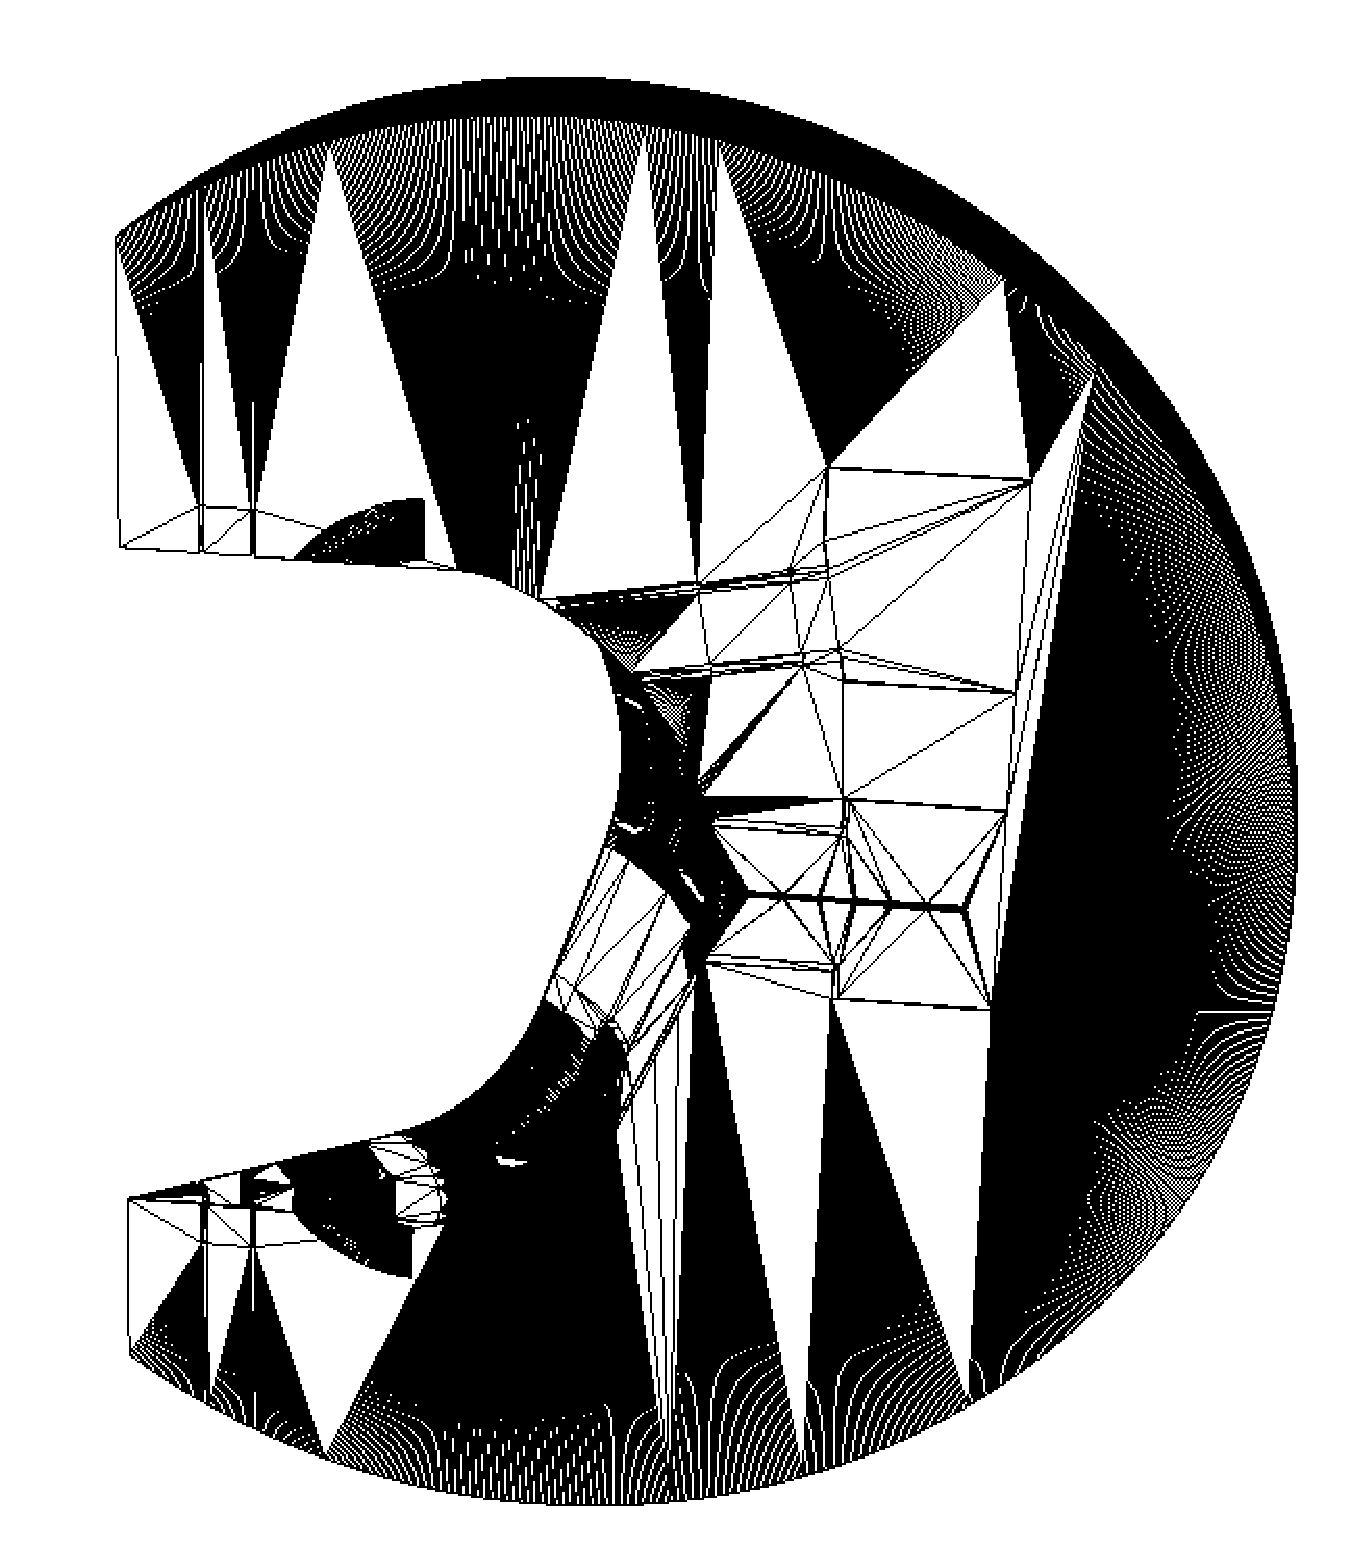
\includegraphics[scale=0.2]{iter_sideon.eps}
  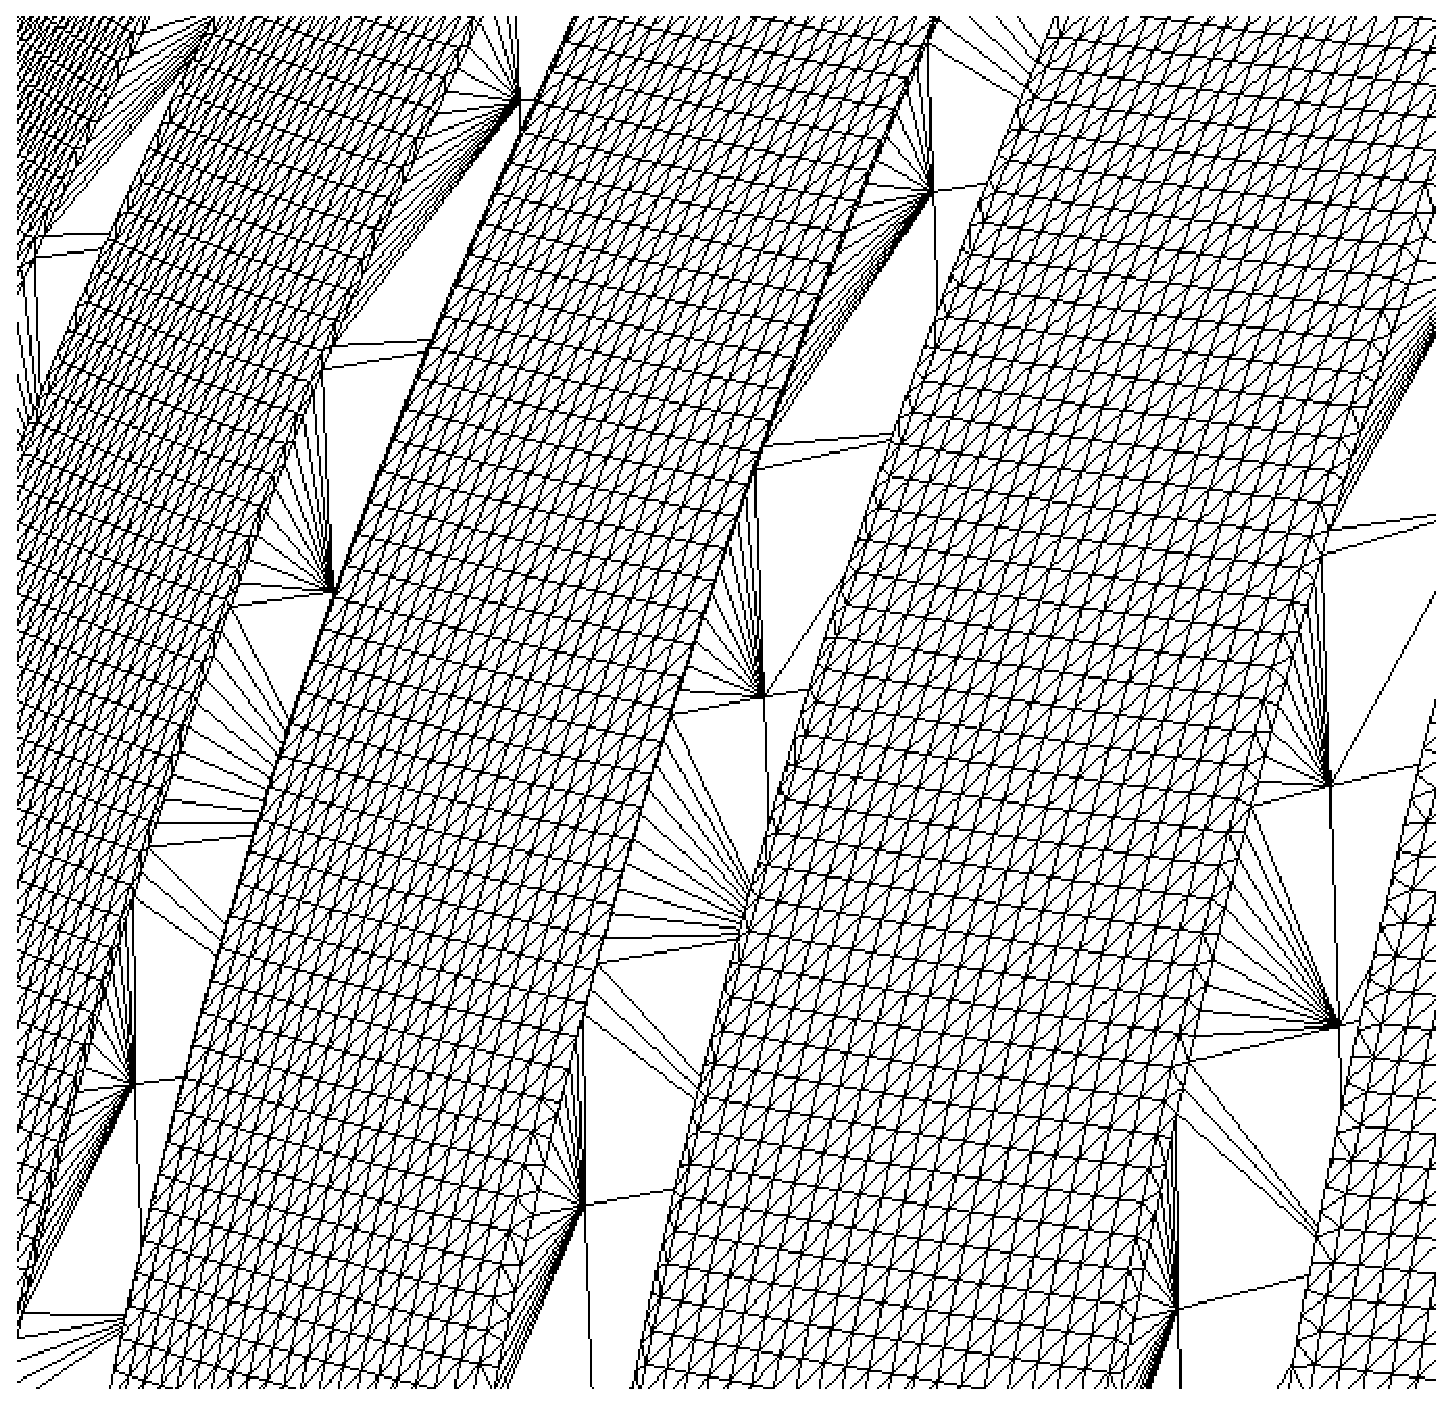
\includegraphics[scale=0.1]{ds_hv.eps}
  \caption{Examples of high valence vertices in analysis and test models.}
  \label{fig:hv_examples}
\end{figure}

These regions are commonly generated in the faceting algorithms used to produce
DAGMC meshes. This faceting scheme (which comes from ACIS libraries underlying
the CUBIT/Trelis graphics engine) is designed to produce the smallest number of
triangles possible to represent the model within the representation tolerance
specified in DAGMC's surface mesh generation preprocessing. This restriction is
favorable to the rasterization process commonly used to display models
interactively in the CAD program. Fewer triangles are better for the purpose
particle tracking in DAGMC as well as long as the geometry is accurately
represented. Even the ideal ray tracing acceleration structure queries for a
given triangle mesh scale as $O(log(N))$, and the size of models being analyzed
using the toolkit provides motivation to keep memory footprints as low as
possible. However, even with fewer triangles undesirable configurations can
impede performance as is shown by a set of tests conducted on models generated
by this faceting scheme.

A study conducted by Steve Jackson in 2010 on the performance of the MOAB ray
tracer revealed a steep degredation in performance with a decreasing faceting
tolerance or an increasing number of triangles. Using a DAGMC-based ray fire
test program, the performance of DAGMC's ray fire ability was evaluated for four
models. These models include a simple sphere, a notched or slotted sphere, and
an outer volume of an ITER model.




